\chapter{Una red neuronal que vuela el dron}
\label{cap:control-neuronal}

\begin{enpocas}
Qué significa que una red neuronal controle los motores, cómo aprende imitando a un experto
(clonación y DAgger), qué es el aprendizaje por refuerzo (PPO), cómo se mete la red en PX4, qué
problemas tuvo la primera versión y cómo se corrigieron.
\end{enpocas}

\section{La idea}

La cascada de PX4 son cuatro controladores encadenados, con decenas de ganancias ajustadas a mano. La
alternativa es \textbf{una sola red neuronal} que reciba el estado del dron y el error de posición y
calcule directamente los cuatro motores. PX4~1.17 trae un módulo para eso, \cod{mc_nn_control}
(\emph{Neural Control}), con una interfaz fija:

\begin{figure}[H]
\centering
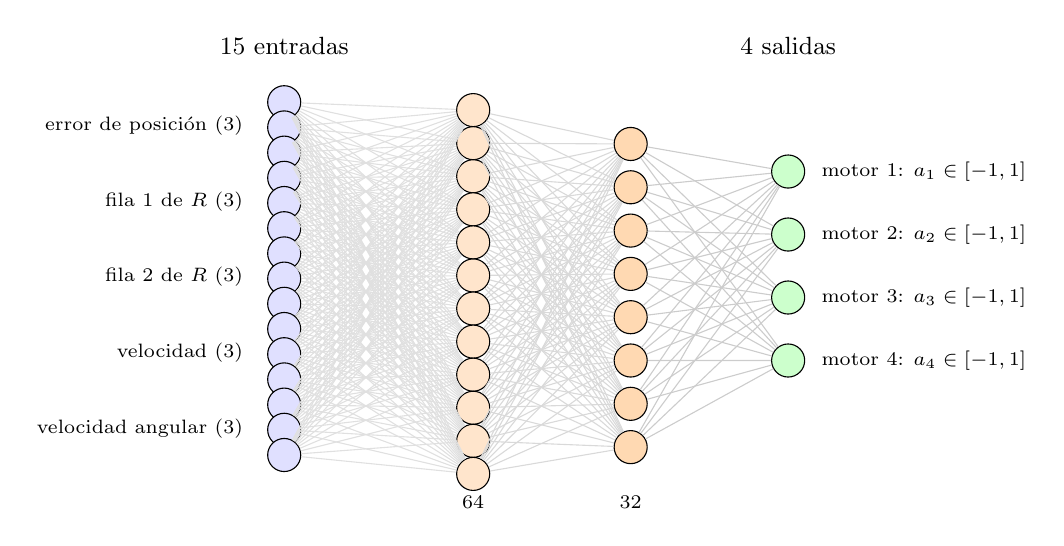
\begin{tikzpicture}[
  n/.style={circle,draw,fill=#1,minimum size=0.42cm,inner sep=0},n/.default=blue!12,
  et/.style={font=\scriptsize,align=right,anchor=east}]
  \foreach \i/\t in {1/{error de posición (3)},4/{fila 1 de $R$ (3)},7/{fila 2 de $R$ (3)},10/{velocidad (3)},13/{velocidad angular (3)}}
    \node[et] at (-0.4,-\i*0.32-0.3) {\t};
  \foreach \i in {1,...,15} \node[n] (a\i) at (0,-\i*0.32) {};
  \foreach \i in {1,...,12} \node[n=orange!20] (b\i) at (2.4,-\i*0.42) {};
  \node at (2.4,-5.4) {\scriptsize 64};
  \foreach \i in {1,...,8} \node[n=orange!30] (c\i) at (4.4,-\i*0.55-0.3) {};
  \node at (4.4,-5.4) {\scriptsize 32};
  \foreach \i in {1,...,4} \node[n=green!20] (d\i) at (6.4,-\i*0.8-0.4) {};
  \foreach \i in {1,...,15} \foreach \j in {1,...,12} \draw[black!12] (a\i) -- (b\j);
  \foreach \i in {1,...,12} \foreach \j in {1,...,8} \draw[black!15] (b\i) -- (c\j);
  \foreach \i in {1,...,8} \foreach \j in {1,...,4} \draw[black!20] (c\i) -- (d\j);
  \foreach \i in {1,...,4} \node[font=\scriptsize,anchor=west] at (6.7,-\i*0.8-0.4) {motor \i: $a_\i\in[-1,1]$};
  \node[font=\small] at (0,0.4) {15 entradas}; \node[font=\small] at (6.4,0.4) {4 salidas};
\end{tikzpicture}
\caption{La red 15-64-32-4 con ReLU: 3\,236 pesos. Entradas en convención ENU-FLU; cada salida se
convierte en la velocidad del motor $\omega_i = \omega_{max}\sqrt{(a_i+1)/2}$.}
\end{figure}

\begin{recuerda}
La red no tiene memoria: en cada instante solo ve el estado actual y el error de posición. No puede
``acumular'' el error como el término integral de un PID. Eso tendrá consecuencias.
\end{recuerda}

\section{Aprender imitando: clonación de comportamiento y DAgger}

¿Cómo se entrena? Lo más directo es \textbf{imitar a un experto}: se vuela con un controlador que ya
funciona (una cascada PD, el ``maestro''), se registran miles de pares (estado, acciones del maestro) y
se entrena la red para que, ante cada estado, dé las mismas acciones. Eso es \textbf{clonación de
comportamiento}, un problema de regresión como cualquier otro.

\begin{ejemplo}
Aprender a manejar viendo a un instructor desde el asiento del copiloto. El problema: el instructor
nunca se sale del carril, así que tú nunca ves cómo se regresa al carril. El día que te desvíes un poco,
no sabrás qué hacer.
\end{ejemplo}

\textbf{DAgger} (\emph{Dataset Aggregation}) resuelve eso: después de la primera ronda, vuela \emph{la
red}, se registran los estados \emph{a los que ella llega} (incluidos sus errores) y el maestro dice qué
habría hecho en cada uno. Se agregan esos ejemplos y se reentrena. Tres rondas bastan. Como el
entrenamiento es en un simulador en Python (el modelo del capítulo de física, a 400~Hz), se agrega
además \textbf{aleatorización de dominio}: en cada episodio la masa, las inercias, $k_f$, el retardo de
los motores y el viento cambian un poco, para que la red no dependa de valores exactos.

\begin{lstlisting}[style=bash]
python3 codigo/nn_imitacion.py --masa 2.114 --com 0.00071 0.00071 --adelanto --salida pesos_nn_x500_busqueda.npz
\end{lstlisting}

\begin{figure}[H]
\centering
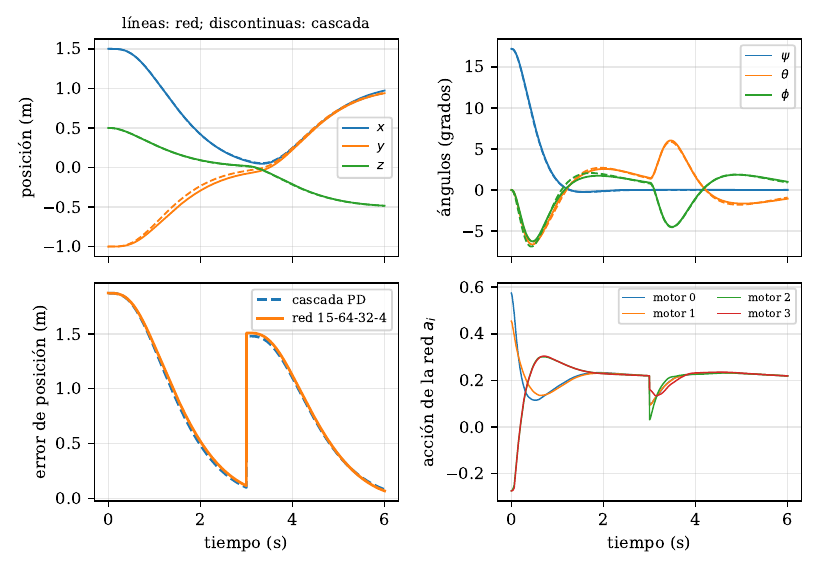
\includegraphics[width=0.85\textwidth]{manual_nn_imitacion_x500_busqueda.png}
\caption{La red (líneas continuas) y el maestro (discontinuas) ante los mismos escalones.}
\end{figure}

\section{Aprender por refuerzo: PPO}

Imitar tiene un techo: la red será, a lo más, tan buena como el maestro. El \textbf{aprendizaje por
refuerzo} quita al maestro: la red prueba acciones, recibe una \textbf{recompensa} (alta si está cerca
del objetivo, baja si se aleja o se estrella) y ajusta sus pesos para aumentar la recompensa acumulada.
\textbf{PPO} (\emph{Proximal Policy Optimization}) es el algoritmo más usado: cambia la política a pasos
pequeños para no destruir lo aprendido. Lleva dos redes: el \emph{actor} (la que vuela) y el
\emph{crítico} (que estima qué tan bueno es cada estado).

La idea del proyecto es partir de la red de imitación y refinarla con PPO
(\cod{codigo/ppo_refinamiento.py}).

\section{De Python a PX4}

\begin{enumerate}
  \item \cod{codigo/exportar_tflite.py} convierte los pesos a \textbf{TensorFlow Lite} (32 bits),
        comprueba que solo use las operaciones que tiene el módulo (capas totalmente conectadas, ReLU y
        suma) y que dé lo mismo que numpy (diferencia de $\sim10^{-6}$), y genera el arreglo en C
        \cod{control_net.cpp/.hpp} (14\,936 bytes).
  \item \cod{scripts/instalar_px4.sh} lo copia a \cod{mc_nn_control} y recompila \cod{px4_sitl_neural}.
  \item La misión cambia al modo \emph{Neural Control} al llegar a la altura de trabajo y regresa a
        offboard antes de aterrizar.
\end{enumerate}
Con ArduPilot, que no tiene un módulo equivalente, la misma red corre en el nodo \cod{controlador_red}
y el plugin \cod{SelectorMotores} deja pasar sus comandos en lugar de los de ArduPilot
(capítulo~\ref{cap:pilotos}).

\begin{leccion}
El diseño original tenía dos detalles que impedían que la red volara: el parámetro
\cod{MC_NN_THRST_COEF} de PX4 trabaja en revoluciones por segundo, no por minuto, y faltaban
\cod{MC_NN_MIN_RPM} y \cod{THR_MDL_FAC}. Con ellos mal, la misma salida de la red producía otro empuje.
Los valores correctos están en el \emph{airframe} \cod{px4/4099_gz_x500_busqueda} y una prueba los
verifica recorriendo toda la cadena de PX4 (red $\rightarrow$ mezclador $\rightarrow$ ESC).
\end{leccion}

\section{Tres problemas de la primera versión y su solución}

\subsection{Un sesgo de 20 cm}

En la primera prueba en SITL quedaba un error permanente en altura de $-0.27$~m: la red se había
entrenado con $m = 2.0$~kg y el x500 completo pesa 2.114~kg. Sin integral, $\Delta z = \Delta m\,g/(m\,k_p)$.
Con la masa correcta el error en altura desapareció, pero quedó un sesgo horizontal de $\approx$0.2~m: la
cámara corre 0.7~mm el centro de masa y la red, que nunca vio ese desequilibrio, se quedaba inclinada
$\approx$1°. La solución fue usar la geometría real en el simulador de entrenamiento (\cod{--com}): el
maestro compensa con los motores y la red aprende a hacerlo.

\subsection{La red iba a la mitad de velocidad}

Una ley PD sin prealimentación, siguiendo una referencia que se mueve a velocidad $v$, se queda atrás
$\frac{k_d}{k_p}v$: con las ganancias del maestro, 4.8~m a 3~m/s. La misión no deja que la consigna se
adelante más de 3~m, así que la red avanzaba a $\approx$1.6~m/s y la misión duraba casi el doble.

La solución clásica de control: mandar una \textbf{consigna adelantada}
\begin{equation}
p_{cons} = p_{ref} + \frac{k_d}{k_p}\,v_{ref}
\quad\Rightarrow\quad
k_p(p_{cons} - p) - k_d v = k_p(p_{ref} - p) + k_d(v_{ref} - v),
\end{equation}
que convierte a la PD en una PD con prealimentación de velocidad, sin cambiar la interfaz de la red.
Pero la red tiene que haber visto esos errores de varios metros: se reentrenó con \cod{--adelanto}
(la mitad de los episodios con referencias que avanzan hasta 4~m/s).

\begin{figure}[H]
\centering
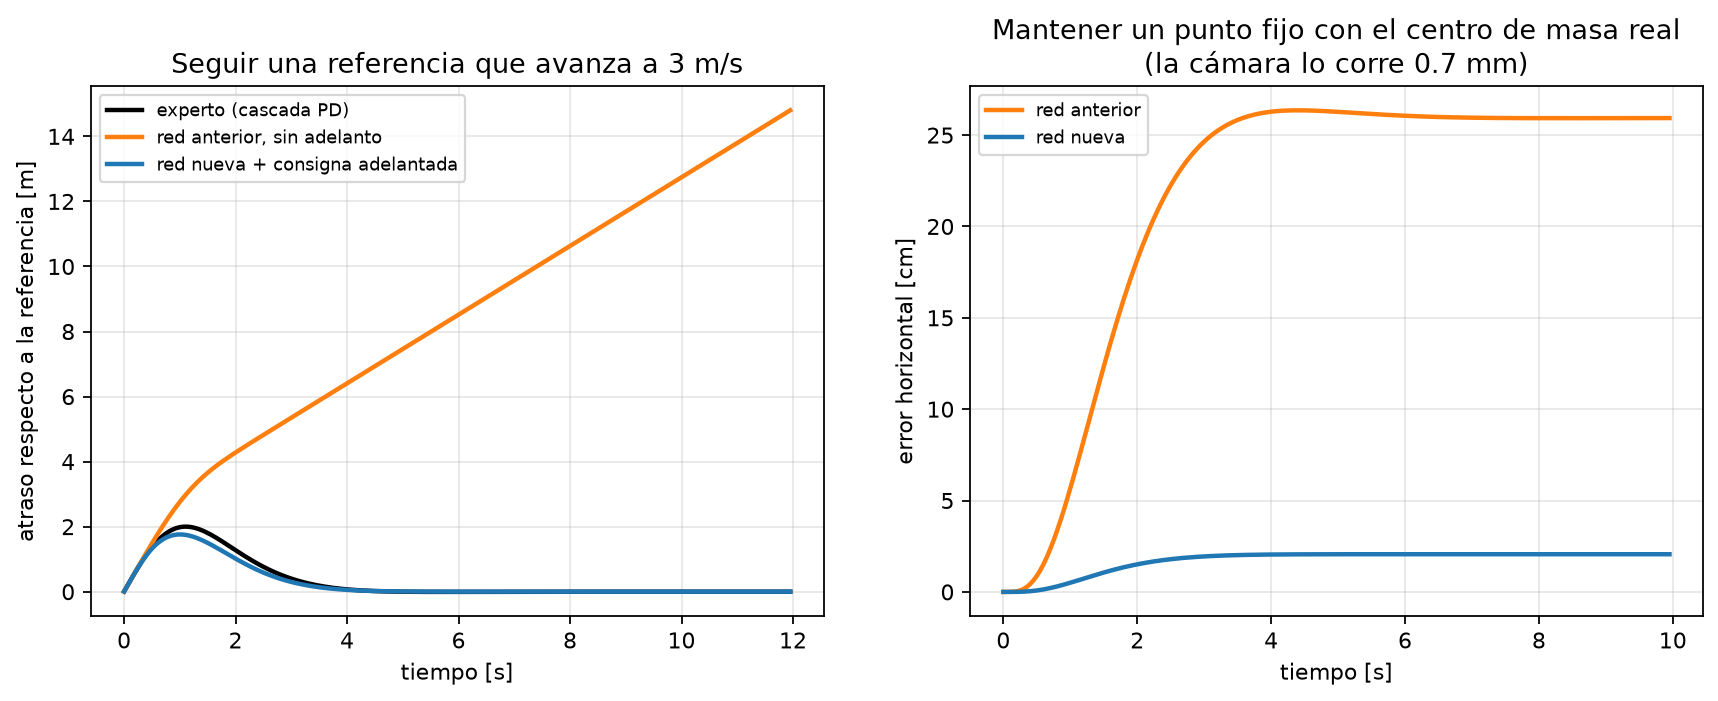
\includegraphics[width=\textwidth]{red_comparacion.png}
\caption{Izquierda: siguiendo una referencia a 3~m/s, la red anterior se atrasa sin parar; la nueva, con
la consigna adelantada, sigue igual que el maestro. Derecha: con el centro de masa real, la red anterior
se queda a 26~cm del punto; la nueva, a 2~cm.}
\end{figure}

\subsection{PPO divergía}

En la primera versión, PPO estaba a la par de la imitación hasta la iteración $\sim$100 y luego se
deterioraba hasta estrellarse en 4 de 40 pruebas. La causa principal estaba en la recompensa original:
cada paso valía $-(|e|^2 + \dots) + 1$, negativo con más de $\sim$1~m de error (hasta $-25$ a 5~m),
mientras que estrellarse costaba solo $-10$ una vez. ¡Terminar pronto ``convenía''! Además los cortes de
episodio por tiempo se trataban como si el dron hubiera fallado, y el crítico, que empieza al azar,
desordenaba la política de imitación en las primeras iteraciones.

La versión mejorada (\cod{--mejorado}) usa una recompensa acotada y positiva mientras el dron vuele,
penaliza estrellarse con $-100$, trata bien los cortes por tiempo, calienta el crítico 15 iteraciones
antes de tocar la política, frena los cambios demasiado grandes (KL) y guarda solo la mejor política.

\begin{figure}[H]
\centering
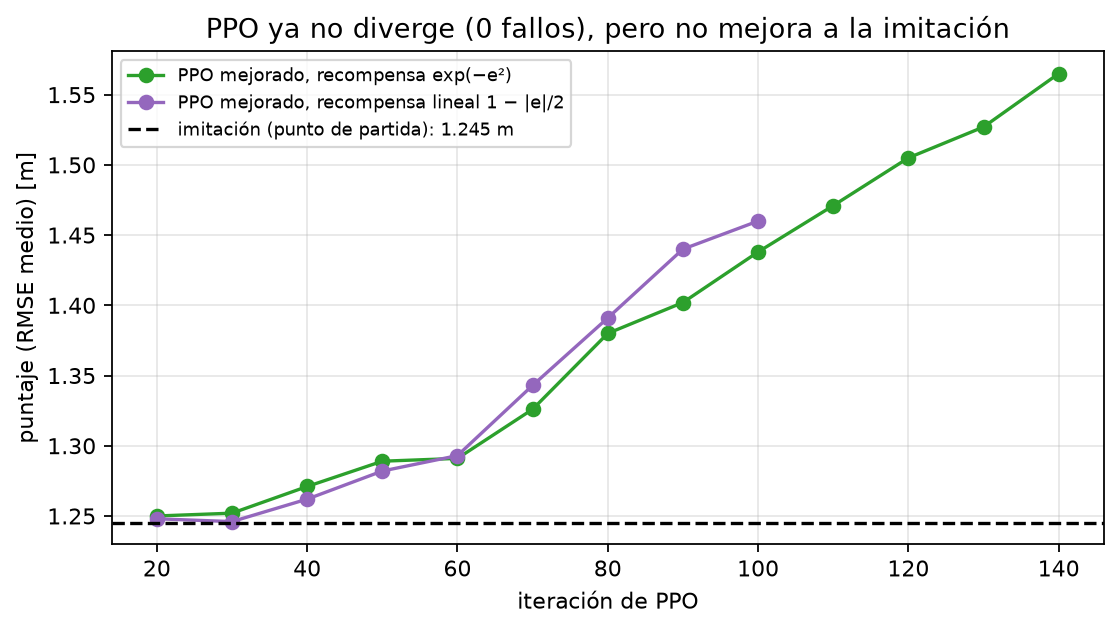
\includegraphics[width=0.8\textwidth]{ppo_curvas.png}
\caption{Con las correcciones PPO ya no diverge (ningún fallo), pero con ninguna de las dos recompensas
probadas mejora a la imitación: se usa la red de imitación.}
\end{figure}

\begin{nota}
Un resultado negativo también es un resultado. Que PPO no mejore aquí es razonable: la red no tiene
memoria y el maestro ya es una buena PD; buena parte del error que queda viene del viento y la masa
aleatorios, que ninguna ley sin integral puede eliminar. Una dirección para mejorarla sería darle a la
red una entrada con el error acumulado, lo que exige modificar el módulo de PX4.
\end{nota}

\section{Resultado en la misión}

\begin{table}[H]
\centering\small
\begin{tabular}{llcccc}
\toprule
\textbf{Piloto} & \textbf{Controlador} & \textbf{Localizadas} & \textbf{Error medio} & \textbf{RMSE ruta} & \textbf{Duración} \\ \midrule
PX4 & cascada & 3/3 & 0.61 m & 0.07 m & 238 s \\
PX4 & red anterior & 3/3 & 0.71 m & 0.11 m & 427 s \\
PX4 & red nueva & 3/3 & 0.52 m & 0.23 m & \textbf{211 s} \\
ArduPilot & red anterior & 3/3 & 0.46 m & 0.12 m & 451 s \\
ArduPilot & red nueva & 3/3 & 0.47 m & 0.19 m & \textbf{240 s} \\
\bottomrule
\end{tabular}
\caption{La misma misión (bosque medio, sol alto, sin viento, 3 personas). Con la red nueva la misión
dura la mitad, igual o menos que con la cascada; sigue la ruta algo peor en las esquinas, donde la
consigna adelantada cambia de dirección de golpe.}
\end{table}
